\section{Generating sound}
After spending a lot of time testing the DAC and figuring out what we could and could not do with the microcontroller and DAC itself, we had to decide on what to implement.

One thing became apparent was that it would not be feasible to do sine wave manipulations on the fly, as floating point operations are slow on the EFM32GG and would not be able to keep up. We instead opted to pre-generate samples of sine waves of different frequencies on a PC. The different samples could then be loaded into the memory on the development board and used to produce sound.

With this setup we can easily create long songs as sequences of reusable notes instead of one long continuous sample. In other words to play the sequence "C D C D C" for 5 seconds we would not need a sequence of five seconds worth of alternating samples, just two short sets of samples, play one for 1 second, then alternate and repeat.

\subsection{Sample generator script}
The sample generator script was written in Python for convenience. It uses a dictionary with note-frequency as key-value pairs, sourced from the equal-tempered scale tuned to $A4 = 440Hz$ \cite{notefreqs}.

The script is fed strings with sequences of note names, a sort of primitive musical sheet, looks up the frequencies of the relevant notes and for each generate samples for one period of a sine wave of that frequency when played at $44.1kHz$. The samples are then scaled and shifted to produce a wave oscillating between \texttt{0} and \texttt{0xFF}.

\begin{figure}[h!]
    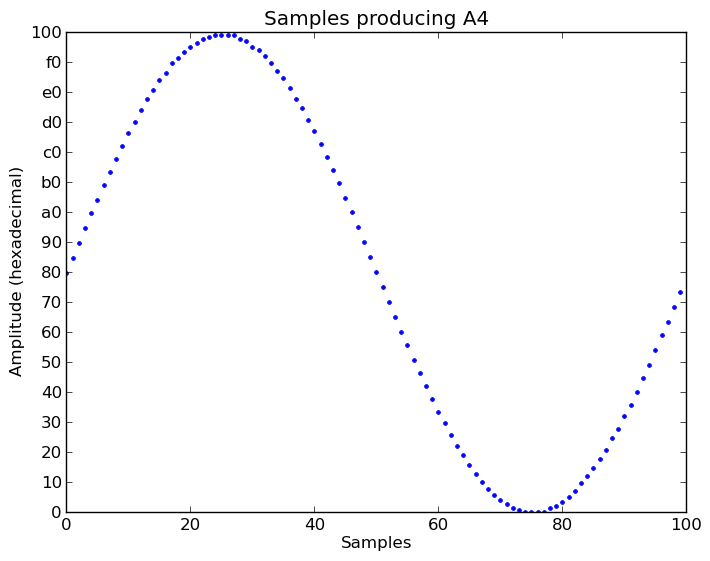
\includegraphics[width=\linewidth]{img/A4.png}
    \caption{Plot of samples producing the note A4 when played at $44.1kHz$}
    \label{fig:A4samples}
\end{figure}


The use of 8 bits instead of 12 was deliberate and seemed entirely advantageous. Since the sine curve the samples produce is so simple, there was no apparent difference in sound quality when decreasing from 12 bit samples to 8 bits. This also allowed us to store the samples as \texttt{uint8\_t} instead of \texttt{uint16\_t}, halving the memory required for storing music.

The script was made to print notes and songs in the form of C structs, as well as supporting variables and functions for playing music. Declarations were written to a header file and implementations to a .c file. The script could then be run directly on the command line, as well as added to the beginning of the \texttt{make run} routine, integrating the python script with the rest of the flashing process.
